\chapter{Introduction}
\label{chapterlabel1}

Real Time Bidding (RTB)\footnote{https://en.wikipedia.org/wiki/Real-time_bidding} has recently become paradigm for online advertising which subversively transformed the whole ecosystem. Unlike traditional contextual advertising, RTB allows advertisers to bid for each of the impression based on user profile data, but not only the contextual web data. Demand side platform (DSP)\footnote{https://en.wikipedia.org/wiki/Demand-side_platform}'s responsibility is to help advertisers optimize their bidding strategy in order to maximize the return of investment (ROI) for its clients. When a potential advertisement audience visits a webpage, a bid request will be sent to DSP who will decide a price to bid for the webspace slot. Economically we know that \(Profit = Revenue - Cost\), in which cost is the winning price for the advertiser, called \textit{Cost-Per-Click} (CPC), revenue, or \textit{Earning per Click} (EPC) is the expected return that can be obtained from the potential advertisement audience based on auction winning function which can be found in \cite{zhang2014optimal}. Briefly speaking, the revenue can be yielded by the product of the expected click per impression and EPC. The pursuit of maximum profit can be achieved by either increasing revenue or decreasing the cost, accurate CTR prediction is crucial to this goal which determines the expected potential revenue for the impression and according bidding price. 

CTR prediction has been researched extensively in recent years academically and industrially, it is especially important to the industry since the CTR prediction impacts the user experience and advertisers' revenue. Microsoft \cite{graepel2010web} has proposed a novel way for CTR prediction model on Sponsored Search in Microsoft’s Bing search engine, Gaussian beliefs across the weights of the model can be maintained and the weights are updated online based on approximate message passing. Facebook \cite{he2014practical} also demonstrates their success on online advertisement CTR prediction. With the combination of decision trees and logistic regression, and other techniques such as feature selection, learning rate schema, data freshness, and data sampling, the performance of CTR prediction can be largely increased.  

However, most current work are restricted to the scope of enhancement of model formation, parameter adjustment and algorithm optimization, but according to Facebook recent report \cite{facebook2015}, the \textit{experimental paradigm is reaching its limits}, in Machine Learning (ML) the experimental paradigm means the procedure of  (i) Setting aside test dataset, (ii) Estimating prediction function using training dataset, and (iii) Measure final performance using testing dataset. In the last a few decades this single paradigm dominates the research in the field of machine learning, which is on the premise that the data used are gathered correctly without bias. In such case, data plays more significant role in enhancing performance of ML application than feature and algorithm, as shown in Figure ~\ref{fig:datai}

\begin{figure}[h]
\centering
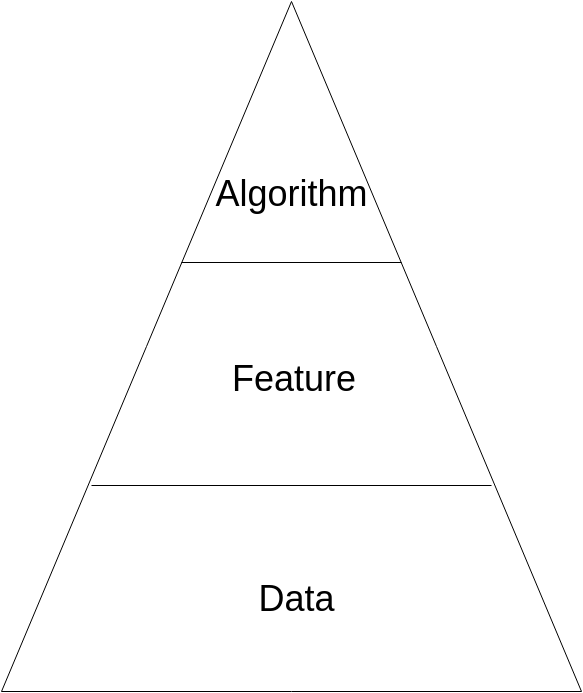
\includegraphics[scale=1.5]{data.png}
\caption{Importance of factors to the performance of ML application}
\label{fig:datai}
\end{figure}

However, in the age of big data \cite{lohr2012age}, large datasets are collected automatically so bias are inevitable among the datasets, therefore, unrealistic results will be obtained from training/testing dataset using the above \textit{experimental paradigm} \cite{torralba2011unbiased}. So for most current researches the models are trained and tested based on one single dataset, the classifiers learned can only work under a certain statistical distribution of the data. Only if with the updates of the model, can the classifiers trained from the old campaigns be applied to new campaigns in the concept of online advertisement. Therefore, under the situation that the advertising data from different advertiser campaigns behave differently and largely biased, according to the idea in \cite{threethings2015} and \cite{domingos2012few}, representation of the data will be essential for machine learning algorithms. More informative data extracted from the dataset, more improvement in performance of the algorithm can be obtained, since digging out the insights from the dataset means filtering out the redundant information which are irrelevant to the prediction task. Therefore, we will focus on the process of \textit{Feature Extraction} or \textit{Feature Engineering} to reach the goal that, 
\begin{itemize}
\item  the new feature space is low dimensional to avoid the \textit{curse of dimensionality} which will be common in the age of \textit{Big Data}
\item the new feature space is informative and the irrelevant data are got rid of, while the performance of prediction task is still comparable to that of traditional binary feature.
\item  the new feature space can help partly solve the \textit{cold start} problem to generalize the model among different campaigns.
\end{itemize}

In this paper we postulate the concept of \textit{Counting Feature} which is the first time, to satisfy the above three requirements. To shortly introduce counting feature, the counting feature of each \textit{field} in the meta ad data is composed of two parts, i.e., \textit{frequency feature} and \textit{average CTR feature}. Frequency feature represents the marginal distribution of the items in the field, and average CTR feature shows the conditional distribution of the clicks on the items in that field. For example, for the field of \textit{City} in meta data there are 500 different cities, if Beijing appears 100,000 times in the dataset with a total number of 1,000,000 impressions, which in total lead to 100 clicks from clients, Hong Kong appears 50,000 times, which also bring 100 clicks for the advertiser. Then in the concept of counting feature, there will be only two features generated from this field of \textit{city}, and the counting values are continuous such as Beijing with frequency counting value 0.1 and average CTR counting value 0.001, Hong Kong with frequency counting value 0.05 and average CTR counting value 0.002. But for binary feature which is encoded into one-hot feature, there will be 500 unique feature generated from the field \textit{city} with only one feature as 1 and others as 0 for each impression, which is sparse and redundant. The goal of low dimension feature space can be achieved by the construction of counting feature based on the statistical property of the dataset. 

What's more, admitting the existence of the bias in the dataset, we prove that the performance of counting feature using non-linear logistic regression model is comparable to that of binary feature using linear logistic regression model. Generally, binary features can be widely used in linear regression based estimators such as logistic regression. Counting features can be used in the tree models such as random forest or gradient boosting regression tree for their continuity property, and they can achieve similar performance in the two situations. To the best of our knowledge, there is no work extensively studying the comparison and relationship of these two kinds of features. Particularly,this is the first time that counting feature based CTR estimation is discussed.  

The classical \textit{Cold Start} problem for online learning is the biggest barrier to meet the 3rd requirement. In the scope of online advertising CTR prediction, cold start problem can be interprated that with the knowledge from old advertisement campaigns, how to apply them to new campaigns which are lack of information initially, in order to avoid repetitive work of data collection and model construction, to make sure that large-scale industry online implementation of CTR prediction system feasible. Most of the current research such as \cite{mohan2011web} \cite{chu2011unbiased} \cite{he2014practical} and \cite{mcmahan2013ad} regard it as an active learning problem, the parameters of the model are regarded as a probability distribution and with the help of Bayesian probit method, the parameters can be updated as new data comes in thus enhancing the precision of CTR prediction for new campaign. However, in the time of big data, online data stream is extremely huge which cost resources and time for the updating of the model. In our work, we try to build a general cross domain model which can be used for each advertisement campaign without the tedious process of model updating. Different from binary feature based model, in which the number of features is variable and feature value is fixed (0 and 1), counting feature benefits from the truth that its number of features is static and feature value can be variable, thus transforming the variability form weight space of the model to the feature space. The counting feature value for each item in each field can be updated with the increasing amount of statistical information gathered from the new campaign. We prove that counting feature performs significantly better than binary feature with high dimensions in terms of cross-domain CTR prediction, the experimental results also show that with the increasing volume of statistical information gathered from new campaign, AUC increases accordingly for counting feature model but with no impact on binary feature based model.

In summary, the contributions of this paper are as follows:
\begin{itemize}
\item We find the relation between binary feature and counting feature and show that their performances for CTR prediction are comparable under certain situation.
\item We research on cross domain learning problem and prove that cold start problem in the field of online advertising CTR prediction is in the scope of \textit{Domain Adaptation} problem. We also show the proofs that only domain distributions differ between old and new advertisement campaigns, the assumption of same task between two campaigns is convincing. 
\item We show that the performance of counting feature in cross domain learning problem for CTR prediction compared to binary feature and validate that counting feature's performance is significantly better than that of binary feature.
\end{itemize}
The rest of the paper is organised as follows, section 2 discusses the related work, our justification of counting feature is formulated in section 3 and in section 4 we discuss on the cross domain problem for online advertisement and model generalization, experiment results are shown in section 5 and we conclude in the last section.

%Inline citation: \bibentry{example-citation}

% This just dumps some pseudolatin in so you can see some text in place.

